\chapter{Testowanie i analiza systemu}

\section{Testy jednostkowe i integracyjne}
Testowanie oprogramowania jest kluczowym elementem zapewnienia jego jakości, stabilności i niezawodności. W ramach niniejszej pracy zastosowano zarówno testy jednostkowe, jak i testy integracyjne w celu weryfikacji poprawności działania poszczególnych modułów systemu oraz ich wzajemnych interakcji.

\subsection{Testy jednostkowe}

Testy jednostkowe koncentrują się na sprawdzaniu poprawności działania pojedynczych funkcji i metod w izolacji. Ich głównym celem jest szybkie wykrywanie błędów w logice aplikacji oraz zapewnienie, że każdy komponent działa zgodnie z oczekiwaniami. Do przeprowadzenia testów jednostkowych zastosowano \textbf{go test}

Przykładowe testy jednostkowe obejmowały:
\begin{itemize}
    \item Sprawdzenie poprawności działania funkcji hashującej hasła użytkowników,
    \item Weryfikację generowania i walidacji tokenów JWT,
    \item Testy funkcji odpowiedzialnych za zarządzanie użytkownikami (dodawanie, edycja, usuwanie),
    \item Weryfikację poprawności operacji CRUD dla bazy danych MongoDB.
\end{itemize}

Wszystkie testy jednostkowe zostały zautomatyzowane i uruchamiane w ramach procesu CI/CD z wykorzystaniem GitHub Actions oraz samodzielnie hostowanych runnerów.

Przeprowadzenie testów jednostkowych umożliwiło rozwój serwisu API bez konieczności posiadania gotowego rozwiązania frontend. Dzięki czemu od samego początku możliwa była weryfikacja oraz wychwycenie błędów logicznych w aplikacji. Takie podejście umożliwia szybki rozwój programu bez obawy o działanie pojedynczych metod i funkcji. Testy jednostkowe nie weryfikują całości działania aplikacji a jedynie indywidualnie jej najmniejsze komponenty. Należy mieć na uwadze, że zgodnie ze sztuką testy jednostkowe powinny nie być zależne od innych metod i funkcji a jeśli dana funkcja lub metoda posiada taką zależność należy ją zasymulować w kodzie poprzez stosowanie tzw. \textbf{Mocków}. Jest to nic innego jak symulowanie działania innej funkcji. Umożliwia ono np. w środowisku testowym uzyskiwać odpowiedzi HTTP poprzez zwracanie stałych odpowiedzi bez konieczności wykonywania zapytań HTTP. Pozwala na integrację z plikami bez fizycznej manipulacji plików. Testy jednostkowe to podstawowy element procesu sprawdzania poprawności oprogramowania. Testów tych powinno być najwięcej zgodnie z paradygmem \textbf{Shift Left}.

\section{Testy wydajnościowe i bezpieczeństwa}
\subsection{Testowanie wydajności systemu}

Testowanie wydajności aplikacji jest kluczowe do zweryfikowania zachowania działania programu pod obciążeniem. Przeprowadzenie takiego testu pozwala na znalezienie tzw. "Wąskich gardeł" programu czyli ścieżek logicznych, które najbardziej obciążają działająca aplikację. Dzięki analizie takich testów możemy odpowiednio nadać wagę zadaniom optymalizacyjnym, żeby poprawić odbiór aplikacji poprzez końcowego użytkownika. Testy wydajnościowe to również testy długoterminowe, dzięki nim można zrozumieć jak aplikacja zachowuje się z długotrwałym obciążeniem i poznać jak reaguje na nagłe skoki obciążenia w różnych momentach czasu działania programu.

Do przeprowadzenia testów wydajnościowych użyty został darmowy program \textbf{ddosify} - jego prosta obsługa oraz konfiguracja, pozwoliła na szybkie jego wdrożenie, a przejrzysty raport wykonania testu na sprawną analizę wydajności programu. 

\subsubsection{Cel testów wydajnościowych}
Celem testów wydajnościowych było:
\begin{itemize}
    \item Ocena wydajności API w warunkach wysokiego obciążenia,
    \item Pomiar czasu odpowiedzi kluczowych endpointów,
    \item Weryfikacja stabilności systemu podczas długotrwałego obciążenia,
    \item Identyfikacja potencjalnych wąskich gardeł aplikacji.
    \item Zweryfikowanie czy w aplikacji nie występują wycieki pamięci podczas długotrwałcyh testów.
\end{itemize}

\subsubsection{Metodyka i analiza testów wydajnościowych}

Testy wydajnościowe zostały przeprowadzone w celu oceny stabilności oraz czasu reakcji systemu backendowego pod rosnącym obciążeniem. Do realizacji testów wykorzystano narzędzie \textbf{Ddosify}, które umożliwia generowanie ruchu HTTP z określoną liczbą żądań oraz mierzenie parametrów takich jak średni czas odpowiedzi, liczba błędów oraz przepustowość systemu. Narzędzie to zostało wybrane ze względu na łatwość integracji oraz możliwość uruchamiania testów z poziomu skryptów bashowych.

Celem testów było:
\begin{itemize}
    \item Określenie, jak system reaguje na wzrastające obciążenie,
    \item Pomiar średniego czasu odpowiedzi dla różnych poziomów liczby zapytań,
    \item Weryfikacja stabilności systemu i pojawiających się błędów przy dużym ruchu,
    \item Wskazanie potencjalnych miejsc wymagających optymalizacji.
\end{itemize}

W ramach testu wykonano serię zapytań do jednego z endpointów API, zwiększając liczbę żądań w krokach od 50 do 500. Dla każdego poziomu obciążenia zarejestrowano średni czas odpowiedzi. Dane zostały zapisane i zwizualizowane w postaci wykresu.

\begin{figure}[H]
    \centering
    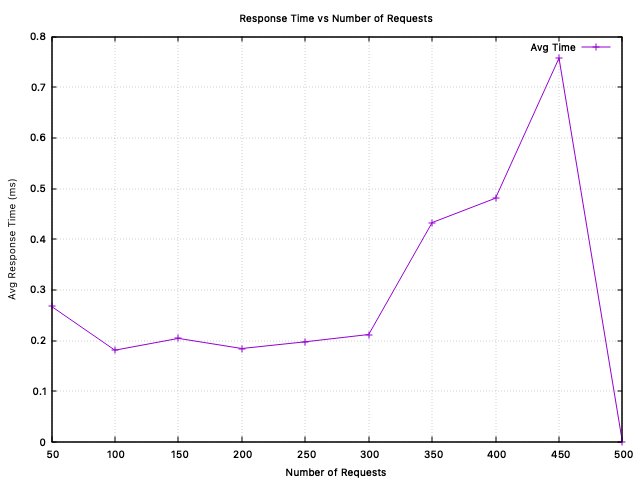
\includegraphics[width=0.9\textwidth]{chapters/assets/wykres czasu odpowiedzi.png}
    \caption{Średni czas odpowiedzi API w zależności od liczby żądań}
\end{figure}

Na powyższym wykresie zauważalna jest względna stabilność średniego czasu odpowiedzi dla zakresu od 50 do około 300 zapytań. W tym przedziale wartości oscylowały wokół 0.18-0.22 ms. Po przekroczeniu 300 żądań widoczny jest wyraźny wzrost opóźnień, a największy skok nastąpił przy 450 żądaniach, gdzie średni czas odpowiedzi osiągnął ponad 0.75 ms. W ostatniej próbie (500 żądań) wszystkie zapytania zakończyły się błędem (500/500 błędów), co skutkowało średnim czasem odpowiedzi równym 0 ms, gdyż odpowiedzi nie zostały zwrócone w ogóle lub zakończyły się błędami.

Za główną przyczynę wystąpienia błędów uznano ograniczenia wydajnościowe bazy danych SQLite, która nie jest przystosowana do obsługi wielu równoczesnych zapytań w środowiskach wysokiego obciążenia. W szczególności brak wsparcia dla wielu jednoczesnych zapisów prowadził do blokowania operacji i przekroczenia limitów czasu odpowiedzi. Dodatkowym czynnikiem była ograniczona liczba zasobów przydzielona aplikacji w środowisku testowym.

\textbf{Wnioski:}
\begin{itemize}
    \item Aplikacja działa stabilnie przy niskim i umiarkowanym obciążeniu (do 300 równoczesnych zapytań),
    \item Wzrost liczby równoczesnych żądań znacząco wpływa na opóźnienia odpowiedzi, co wskazuje na konieczność optymalizacji backendu,
    \item Wystąpienie 100\% błędów przy maksymalnym obciążeniu (500 zapytań) wskazuje na poważne ograniczenie w warstwie komunikacji z bazą danych.
\end{itemize}

\textbf{Rekomendowane działania optymalizacyjne:}
\begin{itemize}
    \item Zastosowanie mechanizmu \textit{connection poolingu} oraz zwiększenie maksymalnej liczby jednoczesnych połączeń do bazy danych,
    \item Wprowadzenie cache'owania odpowiedzi API dla często wywoływanych zapytań,
    \item Refaktoryzacja zapytań do bazy danych - redukcja złożoności oraz optymalizacja indeksów,
    \item Przeprowadzenie testów w środowisku zbliżonym do produkcyjnego z większą wydajnością I/O bazy danych.
\end{itemize}

\noindent
Należy zaznaczyć, że testy wydajnościowe w przedstawionej formie przypominają bardziej atak typu DDoS niż rzeczywiste wykorzystanie systemu przez użytkowników. Mimo to są one niezwykle przydatne w procesie optymalizacji aplikacji - pozwalają zidentyfikować komponenty wymagające poprawy wydajnościowej. Nawet jeśli dana optymalizacja może wydawać się zbędna na etapie prototypowania, warto mieć na uwadze, że zoptymalizowany kod zużywa mniej zasobów systemowych i lepiej skaluje się w środowiskach produkcyjnych.

\subsection{Testowanie bezpieczeństwa aplikacji}

Bezpieczeństwo aplikacji webowych jest jednym z kluczowych aspektów projektowania i wdrażania nowoczesnych systemów. W kontekście niniejszego projektu, który zakłada zarządzanie usługami i użytkownikami, istotne jest zapewnienie odpowiedniego poziomu zabezpieczeń, aby zapobiec nieautoryzowanemu dostępowi, manipulacji danymi oraz wyciekom informacji.

\subsubsection{Zakres testów bezpieczeństwa}

Testowanie bezpieczeństwa przeprowadzono w ograniczonym zakresie, skupiając się na ręcznej weryfikacji najczęściej występujących zagrożeń w aplikacjach webowych, zgodnie z zestawieniem OWASP Top 10. Weryfikacji poddano następujące obszary:

\paragraph{1. Uwierzytelnianie i autoryzacja}
System wykorzystuje tokeny JWT jako mechanizm autoryzacji. W ramach testów:
\begin{itemize}
    \item Sprawdzono odporność logowania na ataki brute-force – nie wykryto możliwości obejścia zabezpieczeń, jednak brak limitu prób logowania może stanowić potencjalne ryzyko.
    \item Zweryfikowano, że po wygaśnięciu tokena nie jest on akceptowany przez serwer.
    \item Potwierdzono, że użytkownicy nieautoryzowani nie mają dostępu do zasobów innych użytkowników.
\end{itemize}

\paragraph{2. Odporność na SQL Injection}
Wszystkie zapytania do bazy danych wykonywane są za pomocą ORM (GORM), co zapewnia parametryzację i zmniejsza ryzyko podatności na SQL Injection. Próby wstrzyknięcia kodu SQL w pola formularzy zakończyły się niepowodzeniem – aplikacja poprawnie odrzucała nieprawidłowe dane wejściowe.

\paragraph{3. Odporność na XSS i CSRF}
\begin{itemize}
    \item Testy XSS (reflected i stored) nie przyniosły rezultatów – aplikacja nie wstrzykuje niezweryfikowanych danych wejściowych do HTML.
    \item Aplikacja wykorzystuje token JWT w nagłówkach, co redukuje ryzyko CSRF, ponieważ brak ciasteczek sesyjnych eliminuje możliwość automatycznego przesyłania uwierzytelnienia.
\end{itemize}

\paragraph{4. Bezpieczeństwo API}
Przeprowadzono testy zabezpieczeń API:
\begin{itemize}
    \item Wszystkie endpointy wymagające autoryzacji poprawnie zwracały kod 401 w przypadku braku lub niewłaściwego tokena.
    \item System nie pozwalał na wykonanie operacji z tokenem innego użytkownika.
    \item Weryfikowano także poprawność nagłówków CORS oraz odpowiedzi serwera na próby nieautoryzowanego dostępu.
\end{itemize}

\paragraph{5. Odporność na przeciążenie (DoS)}
W ramach testów wydajnościowych przeprowadzono symulację ataku DoS:
\begin{itemize}
    \item Wysyłano dużą liczbę zapytań w krótkim czasie – powyżej 400 jednoczesnych zapytań powodowało błędy odpowiedzi serwera.
    \item Błędy te były spowodowane ograniczeniami bazy SQLite, która nie wspiera wielu równoczesnych zapisów.
\end{itemize}

\subsubsection{Rekomendacje i dalsze działania}
Choć aplikacja wykazała odporność na najczęstsze zagrożenia, zaleca się:
\begin{itemize}
    \item Dodanie limitu prób logowania i mechanizmu blokowania IP,
    \item Wdrożenie pełnych testów penetracyjnych (np. z użyciem Burp Suite \cite{BurpSuite} lub OWASP ZAP\cite{ZAP}),
    \item Monitorowanie logów bezpieczeństwa i integracja z systemem alertów,
    \item Przejście na bardziej wydajną bazę danych, wspierającą konkurencyjne zapisy (np. PostgreSQL) w przypadku planowanej produkcyjnej eksploatacji systemu.
\end{itemize}

\textbf{Podsumowanie:} Przeprowadzone testy bezpieczeństwa potwierdzają, że aplikacja w obecnym stanie spełnia podstawowe wymogi bezpieczeństwa, w tym poprawną autoryzację, separację danych użytkowników oraz odporność na podstawowe ataki webowe, takie jak XSS, CSRF czy SQL Injection. Skuteczna implementacja mechanizmu JWT, ochrona endpointów oraz brak dostępu do zasobów bez ważnego tokena świadczą o przemyślanej strukturze kontroli dostępu. Niemniej jednak, dalszy rozwój aplikacji - zwłaszcza w kontekście wdrożenia produkcyjnego - powinien uwzględniać wdrażanie zaawansowanych technik testowania i obrony, takich jak automatyczne testy penetracyjne, analiza statyczna kodu źródłowego, monitorowanie logów pod kątem prób ataków oraz integracja z systemami SIEM (Security Information and Event Management). Rekomendowane jest również regularne wykonywanie audytów bezpieczeństwa oraz testów regresyjnych po każdej większej zmianie kodu lub zależności. Tylko takie podejście pozwoli zapewnić długofalowe bezpieczeństwo systemu oraz ochronę danych użytkowników.